% CorrTrack — v1 vs v2, step by step (with schematics)
% Compile: pdflatex slides_steps_v1_v2.tex
\documentclass[aspectratio=169,10pt]{beamer}
\usepackage[T1]{fontenc}
\usepackage[utf8]{inputenc}
\usepackage{lmodern}
\usepackage{amsmath,amssymb}
\usepackage{tikz}

\setbeamertemplate{navigation symbols}{}
\setbeamertemplate{frametitle}[default][left]
\setbeamerfont{frametitle}{size=\large,series=\bfseries}
\setbeamertemplate{itemize item}{\textcolor{muted}{\textbullet}}

\definecolor{ink}{HTML}{14181F}
\definecolor{accent}{HTML}{2A3A57}
\definecolor{danger}{HTML}{BD3A53}
\definecolor{good}{HTML}{1C8676}
\definecolor{muted}{HTML}{5C6675}

\setbeamercolor{frametitle}{fg=ink}
\setbeamercolor{normal text}{fg=ink}

\newcommand{\vtag}[3]{{\color{#1}\rule{1.8em}{2.2pt}}\; {\ttfamily\small\textbf{\textcolor{#1}{#2}}}\; {\footnotesize #3}\par\vspace{2pt}}
\newcommand{\keydiff}[1]{\noindent\colorbox{accent}{\textcolor{white}{\scriptsize\,\textbf{KEY DIFFERENCE}\,}}\hspace{4pt}{\scriptsize #1}}
\newcommand{\eq}{$\;\equiv\;$}
\tikzset{sc/.style={x=1mm,y=1mm,line width=.5pt,font=\tiny}}

% ---------- schematics ----------
% sketch: window in blocks -> projection -> short vector
\newcommand{\schemaSketch}[2]{\centerline{\begin{tikzpicture}[sc]
  \foreach \i in {0,1,2,3}{\draw[#1] (\i*4,0) rectangle (\i*4+3.4,5);}
  \node[#1,font=\tiny] at (7,-2.2){\ttfamily basic\_window};
  \draw[#1,->] (16.5,2.5)--(21,2.5);
  \draw[#1,fill=#1!12] (21,-1) rectangle (34,6);
  \node[#1,font=\tiny] at (27.5,2.5){#2};
  \draw[#1,->] (34,2.5)--(38,2.5);
  \foreach \i/\h in {0/3,1/5,2/2,3/4,4/3}{\fill[#1] (38.5+\i*1.7,0) rectangle (38.5+\i*1.7+1.2,\h);}
  \node[#1,font=\tiny] at (43,-2.2){sketch};
\end{tikzpicture}}}
% index v1: 1D line + interval
\newcommand{\schemaIndexOneD}{\centerline{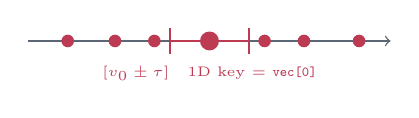
\begin{tikzpicture}[sc]
  \draw[muted,->] (0,0)--(46,0);
  \foreach \x in {5,11,16,30,35,42}{\fill[danger] (\x,0) circle(.8);}
  \draw[danger,line width=1pt] (18,0)--(28,0);
  \draw[danger] (18,-1.6)--(18,1.6);\draw[danger] (28,-1.6)--(28,1.6);
  \fill[danger] (23,0) circle(1.2);
  \node[danger,font=\tiny,below] at (23,-1.9){$[v_0\pm\tau]$ \; 1D key $=$ \texttt{vec[0]}};
\end{tikzpicture}}}
% index v2: 2D cloud + ball
\newcommand{\schemaIndexTwoD}{\centerline{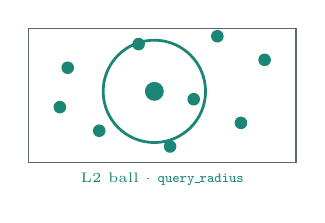
\begin{tikzpicture}[sc]
  \draw[muted] (0,0) rectangle (34,17);
  \foreach \x/\y in {5/12,9/4,14/15,21/8,27/5,30/13,4/7,18/2,24/16}{\fill[good](\x,\y) circle(.8);}
  \fill[good] (16,9) circle(1.2);
  \draw[good,line width=1pt] (16,9) circle(6.5);
  \node[good,font=\tiny] at (17,-2.2){L2 ball · \texttt{query\_radius}};
\end{tikzpicture}}}
% r-axis: v1 keeps everything
\newcommand{\schemaAxisFull}{\centerline{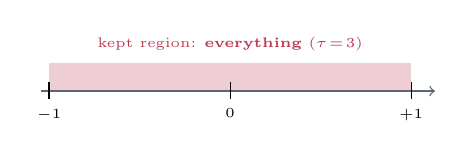
\begin{tikzpicture}[sc]
  \fill[danger!25] (0,0) rectangle (46,3.5);
  \draw[muted,->] (-1,0)--(49,0);
  \foreach \x/\l in {0/{$-1$},23/{$0$},46/{$+1$}}{\draw (\x,-1)--(\x,1.2);\node[font=\tiny,below] at (\x,-1){\l};}
  \node[danger,font=\tiny] at (23,6){kept region: \textbf{everything} $(\tau\!=\!3)$};
\end{tikzpicture}}}
% r-axis: v2 keeps [0.7,1]
\newcommand{\schemaAxisPart}{\centerline{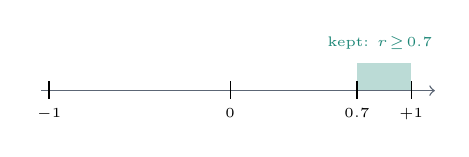
\begin{tikzpicture}[sc]
  \fill[good!30] (39.1,0) rectangle (46,3.5);
  \draw[muted,->] (-1,0)--(49,0);
  \foreach \x/\l in {0/{$-1$},23/{$0$},39.1/{$0.7$},46/{$+1$}}{\draw (\x,-1)--(\x,1.2);\node[font=\tiny,below] at (\x,-1){\l};}
  \node[good,font=\tiny] at (42,6){kept: $r\!\ge\!0.7$};
\end{tikzpicture}}}
% Pearson gauge
\newcommand{\schemaGauge}[1]{\centerline{\begin{tikzpicture}[sc]
  \draw[#1,fill=#1!12] (0,0) rectangle (46,3);
  \fill[#1!45] (41.4,0) rectangle (46,3);
  \draw[#1,line width=1pt] (41.4,-1)--(41.4,4.5);
  \node[#1,font=\tiny,above] at (41.4,4){$r\!\ge\!0.8$};
  \node[font=\tiny,below] at (0,0){$-1$};\node[font=\tiny,below] at (23,0){$r$};\node[font=\tiny,below] at (46,0){$+1$};
\end{tikzpicture}}}
% monitoring timeline
\newcommand{\schemaTimeline}[1]{\centerline{\begin{tikzpicture}[sc]
  \draw[muted,->] (0,0)--(48,0);\node[font=\tiny,below] at (47,0){$t$};
  \fill[#1!30] (9,1.5) rectangle (31,4.5);\draw[#1] (9,1.5) rectangle (31,4.5);
  \node[#1,font=\tiny] at (6,3){$\blacktriangle$};\node[#1,font=\tiny,below] at (9,1.3){in};
  \draw[#1,dashed] (20,0)--(20,7);\node[#1,font=\tiny,above] at (20,5.4){\texttt{sign\_flip}};
  \node[#1,font=\tiny] at (34,3){$\blacktriangledown$};\node[#1,font=\tiny,below] at (31,1.3){out};
\end{tikzpicture}}}

\begin{document}
\footnotesize

% ===== 1. SKETCH =====
\begin{frame}[t]{Step 1 — Sketch: projecting the window \; · \; v1 vs v2}
\footnotesize
\emph{Role} --- turn each window into a short vector ($n\_vectors$) that \textbf{preserves correlation} (Johnson–Lindenstrauss projection).
\vspace{3pt}
\begin{columns}[t]
\begin{column}{0.5\textwidth}
\vtag{danger}{v1}{random projection, 1 method}
\schemaSketch{danger}{$R=\pm1$}
\vspace{6pt}
{\scriptsize\begin{itemize}\setlength\itemsep{2pt}
\item \textbf{Rademacher} matrix $\pm1/\sqrt{n\_vectors}$ $+$ \texttt{toggleVector} (order)
\item incremental via \texttt{basicDots}
\item normalization \texttt{z} $|$ \texttt{mean\_l2} · Cython kernel
\end{itemize}}
\end{column}
\begin{column}{0.5\textwidth}
\vtag{good}{v2}{v1 port $+$ 4 more methods}
\schemaSketch{good}{$R=N(0,1)$}
\vspace{6pt}
{\scriptsize\begin{itemize}\setlength\itemsep{2pt}
\item Gaussian $N(0,1)$ $+$ \texttt{znormalize}
\item \textbf{5 methods}: RP, \texttt{fft\_lowpass/topk}, \texttt{median\_blocks/phase}
\item \texttt{project} is \textbf{backend-swappable}
\end{itemize}}
\end{column}
\end{columns}
\vspace{4pt}
\keydiff{the v2 sketch is \textbf{generalized} (incl. lag-invariant FFT) and \textbf{swappable} $\to$ it becomes a \textbf{separability lever}, not a constant.}
\end{frame}

% ===== 2. INDEX =====
\begin{frame}[t]{Step 2 — Index / neighbor retrieval \; · \; v1 vs v2}
\footnotesize
\emph{Role} --- for each window, find its neighbors in sketch space (\textbf{raw candidates}).
\vspace{3pt}
\begin{columns}[t]
\begin{column}{0.5\textwidth}
\vtag{danger}{v1}{1 structure, 1D key}
\schemaIndexOneD
\vspace{7pt}
{\scriptsize\begin{itemize}\setlength\itemsep{2pt}
\item \texttt{bptree} (sorted list) or \texttt{flat}
\item range $[v_0\pm\tau]$ \textbf{then} full-L2 refine (\texttt{find\_pairs\_full})
\item \texttt{neg\_corr} $\to$ also inserts $-vec$
\end{itemize}}
\end{column}
\begin{column}{0.5\textwidth}
\vtag{good}{v2}{13 indexes, isolated retrieval}
\schemaIndexTwoD
\vspace{2pt}
{\scriptsize\begin{itemize}\setlength\itemsep{2pt}
\item \textbf{13 indexes}: grid / bst / kdtree / hnsw / annoy …
\item \texttt{query\_batch} $=$ \textbf{BLAS cdist} (tree off in batch)
\item \texttt{query\_radius} · grid = multi-table LSH
\end{itemize}}
\end{column}
\end{columns}
\vspace{4pt}
\keydiff{v1 $=$ one 1D structure \emph{welded} to selection; v2 $=$ 13 \textbf{interchangeable} indexes, retrieval \textbf{isolated}.}
\end{frame}

% ===== 3. SELECTION <-> GATE =====
\begin{frame}[t]{Step 3 — Selection (v1) \eq Index$+$Gate (v2): the bridge}
\footnotesize
\emph{Role} --- decide which pairs deserve exact validation. \emph{Same $r$-axis below: what each version keeps.}
\vspace{2pt}
\begin{columns}[t]
\begin{column}{0.5\textwidth}
\vtag{danger}{v1}{euclidean radius, unbounded}
\schemaAxisFull
\vspace{7pt}
{\scriptsize\begin{itemize}\setlength\itemsep{2pt}
\item filter $=$ \texttt{cell\_size} $(\tau)$: $r\gtrsim 1-\tau^2/2$
\item vote \texttt{freq\_threshold}; $=0$ in full\_vector (default)
\item \textbf{1 knob}, couples retrieval/filter · $\tau>2\Rightarrow$ keeps all
\end{itemize}}
\end{column}
\begin{column}{0.5\textwidth}
\vtag{good}{v2}{cosine, bounded}
\schemaAxisPart
\vspace{7pt}
{\scriptsize\begin{itemize}\setlength\itemsep{2pt}
\item retrieval \texttt{query\_radius} \emph{separate} from filter
\item gate \texttt{sketch\_threshold}: $\cos\!\approx\!r$, \textbf{bounded} $[-1,1]$
\item \texttt{neg\_corr} $\to |\cos|$
\end{itemize}}
\end{column}
\end{columns}
\vspace{2pt}
\centerline{\scriptsize same $r$ (JL) --- setting \texttt{sketch\_threshold}$=1-\tau^2/2$ reproduces the v1 filter \emph{exactly}}
\vspace{2pt}
\keydiff{v2 \textbf{decouples} retrieval and filtering \emph{and} bounds the threshold $\to$ v1's ``keep everything'' becomes \textbf{inexpressible}.}
\end{frame}

% ===== 4. VALIDATION =====
\begin{frame}[t]{Step 4 — Exact Pearson validation \; · \; v1 vs v2}
\footnotesize
\emph{Role} --- \textbf{exact} correlation on raw windows: confirm or reject each candidate.
\vspace{3pt}
\begin{columns}[t]
\begin{column}{0.5\textwidth}
\vtag{danger}{v1}{Pearson $+$ guards}
\schemaGauge{danger}
\vspace{7pt}
{\scriptsize\begin{itemize}\setlength\itemsep{2pt}
\item \texttt{fast\_corr\_and\_dist} ($+$ \texttt{min\_dist})
\item rejects: std$<10^{-3}$ \textbf{and} \textbf{spiked} (kurtosis$>5$)
\item Cython batch, threads
\end{itemize}}
\end{column}
\begin{column}{0.5\textwidth}
\vtag{good}{v2}{batch Pearson $+$ backend}
\schemaGauge{good}
\vspace{7pt}
{\scriptsize\begin{itemize}\setlength\itemsep{2pt}
\item \texttt{backend.correlate} per batch (swappable)
\item reject: \texttt{std\_threshold} only (\textbf{no} kurtosis)
\item returns the \textbf{signed lag} ($t_A-t_B$)
\end{itemize}}
\end{column}
\end{columns}
\vspace{4pt}
\keydiff{same Pearson; v1 adds an anti-spike (kurtosis) $+$ \texttt{min\_dist}; v2 $=$ \texttt{std\_threshold} only, swappable backend, native signed lag.}
\end{frame}

% ===== 5. MONITORING =====
\begin{frame}[t]{Step 5 — Persistence monitoring \; · \; v1 vs v2}
\footnotesize
\emph{Role} --- track over time the \textbf{lifetime} of correlations and their \textbf{anomalies} (onset, drop, sign change).
\vspace{3pt}
\begin{columns}[t]
\begin{column}{0.5\textwidth}
\vtag{danger}{v1}{coupled to compute $+$ artifacts}
\schemaTimeline{danger}
\vspace{6pt}
{\scriptsize\begin{itemize}\setlength\itemsep{2pt}
\item \texttt{corr\_lengths} / \texttt{corr\_anomalies}, key $(id_1,id_2,\text{lag})$
\item \texttt{\_in\_corr} $+$ \texttt{\_out\_corr}, Cython kernel
\item coupled to artifact writing (disk spill)
\end{itemize}}
\end{column}
\begin{column}{0.5\textwidth}
\vtag{good}{v2}{pure bookkeeping}
\schemaTimeline{good}
\vspace{6pt}
{\scriptsize\begin{itemize}\setlength\itemsep{2pt}
\item \texttt{Monitor} class: \texttt{active} / \texttt{episodes}
\item typed anomalies: \texttt{in} / \texttt{out} / \texttt{sign\_flip}
\item \textbf{no backend dependency}
\end{itemize}}
\end{column}
\end{columns}
\vspace{4pt}
\keydiff{same model (lifetime $+$ anomalies); v2 is \textbf{decoupled} from compute and artifacts, where v1 mixes Cython kernel and disk spill.}
\end{frame}

\end{document}
